% =====================================================================
%  Relatório Técnico — Trabalho de Sistemas Operacionais
%  Compilar dentro desta pasta: pdflatex relatorio.tex (duas vezes)
%  No Overleaf: envie este arquivo e as imagens da pasta docs/.
% =====================================================================
\documentclass[12pt,a4paper]{article}

% ---------------------------------------------------------------------
%  PREENCHA OS DADOS DO GRUPO AQUI
% ---------------------------------------------------------------------
\newcommand{\instituicao}{NOME DA INSTITUIÇÃO}
\newcommand{\curso}{Curso de Graduação em ...}
\newcommand{\disciplina}{Sistemas Operacionais}
\newcommand{\professor}{Nome do(a) Professor(a)}
\newcommand{\integrantes}{%
  Nome do Integrante 1\\
  Nome do Integrante 2\\
  Nome do Integrante 3}
\newcommand{\cidade}{Cidade -- UF}
\newcommand{\ano}{2026}
\newcommand{\repositorio}{https://github.com/julianoreis27/trabalho-so}
% Endereço gerado pelo Cloud Run depois da publicação (passo 6 do README)
\newcommand{\urlaplicacao}{https://estoque-XXXXXXXX.southamerica-east1.run.app}
% ---------------------------------------------------------------------

\usepackage[utf8]{inputenc}
\usepackage[T1]{fontenc}
\usepackage[brazil]{babel}
\usepackage{lmodern}
\usepackage{microtype}
\usepackage[top=3cm,left=3cm,right=2cm,bottom=2cm]{geometry}
\usepackage{setspace}
\usepackage{indentfirst}
\usepackage{graphicx}
\usepackage{float}
\usepackage{booktabs}
\usepackage{tabularx}
\usepackage{array}
\usepackage{enumitem}
\usepackage{xcolor}
\usepackage{listings}
\usepackage{caption}
\usepackage{tikz}
\usetikzlibrary{arrows.meta}
\usepackage{xurl}
\usepackage[hidelinks]{hyperref}

\onehalfspacing
\setlength{\parindent}{1.25cm}
\setlist{itemsep=2pt,topsep=4pt}
\captionsetup{font=small,labelfont=bf}
\graphicspath{{../}}

\definecolor{verde}{HTML}{0F7B4B}
\definecolor{cinzacod}{HTML}{F4F6F8}
\definecolor{comentario}{HTML}{5C6B78}

\lstdefinelanguage{JavaScript}{
  keywords={const,let,var,function,return,if,else,for,while,new,class,async,await,throw,try,catch,require},
  sensitive=true,
  comment=[l]{//},
  morecomment=[s]{/*}{*/},
  morestring=[b]',
  morestring=[b]",
  morestring=[b]`,
}
\lstset{
  basicstyle=\ttfamily\footnotesize,
  keywordstyle=\color{verde}\bfseries,
  commentstyle=\color{comentario}\itshape,
  stringstyle=\color{orange!70!black},
  backgroundcolor=\color{cinzacod},
  frame=single,
  rulecolor=\color{black!15},
  breaklines=true,
  columns=fullflexible,
  keepspaces=true,
  showstringspaces=false,
  captionpos=b,
  literate=
    {á}{{\'a}}1 {é}{{\'e}}1 {í}{{\'i}}1 {ó}{{\'o}}1 {ú}{{\'u}}1
    {Á}{{\'A}}1 {É}{{\'E}}1 {Í}{{\'I}}1 {Ó}{{\'O}}1 {Ú}{{\'U}}1
    {ã}{{\~a}}1 {õ}{{\~o}}1 {Ã}{{\~A}}1 {Õ}{{\~O}}1
    {â}{{\^a}}1 {ê}{{\^e}}1 {ô}{{\^o}}1 {à}{{\`a}}1
    {ç}{{\c c}}1 {Ç}{{\c C}}1,
}
\renewcommand{\lstlistingname}{Código}

\newcommand{\arq}[1]{\texttt{#1}}
\newcommand{\cab}[1]{\textbf{\begin{tabular}[b]{@{}c@{}}#1\end{tabular}}}

\begin{document}

% =====================================================================
%  CAPA
% =====================================================================
\begin{titlepage}
  \begin{center}
    {\large\bfseries \MakeUppercase{\instituicao}}\\[4pt]
    {\large \curso}\\[2pt]
    {\large Disciplina: \disciplina}

    \vspace{2.6cm}
    {\large \integrantes}

    \vfill
    {\LARGE\bfseries Estoque do Supermercado}\\[12pt]
    {\Large Sistema web de controle de estoque hospedado no Google Cloud}\\[16pt]
    {\large Relatório técnico do trabalho prático}

    \vfill
    \begin{flushright}
      \begin{minipage}{0.55\textwidth}
        \small\singlespacing
        Relatório apresentado à disciplina de \disciplina, ministrada por \professor,
        como requisito parcial de avaliação.
      \end{minipage}
    \end{flushright}

    \vspace{2cm}
    {\large \cidade}\\[2pt]
    {\large \ano}
  \end{center}
\end{titlepage}

\tableofcontents
\clearpage

% =====================================================================
\section{Tema e descrição do projeto}
% =====================================================================

O tema do projeto é um \textbf{sistema web de controle de estoque de supermercado}. Pelo
navegador, o usuário cadastra, consulta, edita e exclui produtos, registra entradas e saídas
de mercadorias e acompanha indicadores como o valor total em estoque, os itens abaixo do
estoque mínimo e os produtos que vencem nos próximos sete dias.

A aplicação foi reaproveitada do trabalho da disciplina de Computação em Nuvem, como o
enunciado permite. Para este trabalho ela foi enxugada e adaptada: saíram os arquivos de
implantação na AWS e o banco DynamoDB, o PostgreSQL passou a ser o único banco de dados e a
aplicação foi preparada para ser hospedada no \textbf{Google Cloud}, em um contêiner no
\textbf{Cloud Run} com o banco no \textbf{Cloud SQL}.

O sistema depende do sistema operacional em pontos concretos. Vários caixas podem dar baixa
no mesmo produto ao mesmo tempo, o que cria uma \textbf{condição de corrida}. O servidor
precisa reagir aos \textbf{sinais} que o Cloud Run envia ao desligar um contêiner. A
aplicação conversa com o banco por um \textbf{socket Unix}. E ela roda como um
\textbf{processo} isolado dentro de um contêiner. A Seção~\ref{sec:conceitos} detalha cada um
desses pontos.

O código-fonte está em \url{\repositorio}.

% =====================================================================
\section{Objetivo}
% =====================================================================

\textbf{Objetivo geral:} disponibilizar um sistema de controle de estoque funcional,
hospedado na nuvem, e mostrar como os mecanismos do sistema operacional influenciam
diretamente a execução e a administração dessa aplicação.

\textbf{Objetivos específicos:}
\begin{enumerate}
  \item Oferecer o cadastro completo de produtos e o controle de entradas e saídas de estoque.
  \item Garantir que vendas simultâneas do mesmo produto nunca deixem o estoque negativo nem
        percam atualizações, aplicando exclusão mútua.
  \item Encerrar o servidor de forma graciosa ao receber os sinais \texttt{SIGTERM} e
        \texttt{SIGINT}, sem interromper requisições em andamento.
  \item Empacotar a aplicação em um contêiner e prepará-la para o Google Cloud Run, com
        o banco no Cloud SQL.
\end{enumerate}

% =====================================================================
\section{Metodologia}
% =====================================================================

\subsection{Etapas do desenvolvimento}

\begin{enumerate}
  \item \textbf{Reaproveitamento.} O código do sistema de estoque (API REST, validação e
        interface web) foi trazido do projeto de Computação em Nuvem.
  \item \textbf{Limpeza.} Foram removidos o template CloudFormation, o diagrama da arquitetura
        AWS, o repositório DynamoDB e as dependências do SDK da AWS. O PostgreSQL, que o
        sistema já suportava, passou a ser o único banco.
  \item \textbf{Adaptação para o Google Cloud.} Foram criados o \arq{Dockerfile} e os arquivos
        \arq{.dockerignore} e \arq{.gcloudignore}; a conexão com o banco passou a aceitar o
        socket Unix do Cloud SQL; o servidor passou a registrar o sinal recebido no encerramento;
        e o pool de conexões ganhou um tratador de erros, para que uma conexão derrubada pelo
        banco não encerre o processo.
  \item \textbf{Testes.} Os testes de integração foram adaptados para o PostgreSQL e ganharam
        um caso com 100 saídas simultâneas do mesmo produto.
  \item \textbf{Verificação.} A imagem do contêiner foi construída e executada localmente
        nas mesmas condições do Cloud Run, e os experimentos da Seção~\ref{sec:resultados}
        foram realizados.
\end{enumerate}

\subsection{Funcionalidades implementadas}

\begin{itemize}
  \item Cadastro, listagem, consulta, edição e exclusão de produtos, com nome, categoria,
        código de barras, quantidade, unidade, estoque mínimo, preço unitário, validade e
        fornecedor.
  \item Entrada e saída de estoque como operação atômica, que impede estoque negativo.
  \item Painel de resumo: total de produtos, itens em estoque, valor total, itens abaixo do
        mínimo e produtos que vencem em até 7 dias.
  \item Busca por nome, fornecedor ou código de barras (ignorando acentos) e filtros por
        categoria e situação (estoque baixo, vencendo).
  \item Indicação da situação de cada produto: OK, estoque baixo, sem estoque, vence em breve
        ou vencido.
  \item Validação dos dados no servidor, com mensagens de erro exibidas ao lado de cada campo.
  \item API REST com rota de verificação de saúde (\texttt{/api/health}).
\end{itemize}

\subsection{Arquitetura e hospedagem}

A Figura~\ref{fig:arquitetura} mostra a arquitetura no Google Cloud. O navegador acessa o
endereço público do serviço no \textbf{Cloud Run}, que executa o contêiner da aplicação e cria
ou remove instâncias conforme o número de acessos (no máximo duas, neste projeto). Cada
instância é um processo Node.js que serve tanto a interface web quanto a API. O banco é um
PostgreSQL 16 gerenciado pelo \textbf{Cloud SQL}; o Cloud Run disponibiliza, dentro do
contêiner, um socket Unix em \texttt{/cloudsql/PROJETO:REGIAO:INSTANCIA} e encaminha as
conexões feitas nele até a instância do banco. O endereço do banco, que contém a senha, fica
no \textbf{Secret Manager} e é entregue ao processo como a variável de ambiente
\texttt{DATABASE\_URL}.

\begin{figure}[H]
\centering
\begin{tikzpicture}[
    font=\small,
    caixa/.style={draw, rounded corners=3pt, align=center, minimum height=1.0cm, fill=white},
    seta/.style={-{Latex[length=2.2mm]}, thick}]

  \node[caixa, minimum width=3.4cm] (nav) at (0, 0) {Navegador};
  \node[caixa, text width=4.6cm, fill=verde!8, draw=verde!70!black] (run) at (0, -2.6)
      {\textbf{Cloud Run}\\ contêiner com o processo\\ \texttt{node src/server.js} (PID 1)};
  \node[caixa, minimum width=6.2cm, fill=orange!10, draw=orange!70!black] (sql) at (0, -5.6)
      {\textbf{Cloud SQL} -- PostgreSQL 16\\ banco \texttt{estoque}, tabela \texttt{produtos}};
  \node[caixa, text width=3.3cm, fill=blue!6, draw=blue!50!black] (sec) at (5.9, -2.6)
      {\textbf{Secret Manager}\\ \texttt{DATABASE\_URL}};
  \node[caixa, text width=3.3cm, fill=black!4] (cb) at (-5.9, -2.6)
      {\textbf{Cloud Build}\\ gera a imagem do \texttt{Dockerfile}};

  \draw[seta] (nav) -- node[right] {HTTPS} (run);
  \draw[seta] (run) -- node[right, align=left] {socket Unix\\\texttt{/cloudsql/...}} (sql);
  \draw[seta] (sec) -- node[above, font=\scriptsize] {variável} (run);
  \draw[seta] (cb) -- node[above, font=\scriptsize] {imagem} (run);
\end{tikzpicture}
\caption{Arquitetura da aplicação hospedada no Google Cloud.}
\label{fig:arquitetura}
\end{figure}

A publicação é feita com o comando \texttt{gcloud run deploy -{}-source .}, que envia o código ao
\textbf{Cloud Build}, gera a imagem a partir do \arq{Dockerfile} e a publica no Cloud Run. O
passo a passo completo (criação do banco, do segredo, das permissões e a publicação) está no
\arq{README.md} do repositório. Endereço da aplicação publicada: \url{\urlaplicacao}.

Para desenvolvimento, a mesma aplicação roda no computador com um PostgreSQL local criado pelo
\arq{docker-compose.yml}.

\subsection{Tecnologias utilizadas}

\begin{description}[style=nextline,leftmargin=0.6cm]
  \item[Linguagem de programação] \textbf{JavaScript}, executado no \textbf{Node.js 22} no
        servidor e no navegador no front-end, junto com HTML e CSS.
  \item[Banco de dados] \textbf{PostgreSQL 16}: no \textbf{Google Cloud SQL} em produção e em
        um contêiner Docker no desenvolvimento. Uma tabela, \texttt{produtos}, criada
        automaticamente na inicialização.
  \item[Frameworks] \textbf{Express 5} no back-end, para as rotas da API REST e os arquivos
        estáticos. O front-end não usa framework.
  \item[Bibliotecas] As do Node.js listadas na Tabela~\ref{tab:bibliotecas}.
  \item[Infraestrutura] \textbf{Docker} (imagem \texttt{node:22-slim}), \textbf{Google Cloud
        Run}, \textbf{Cloud SQL}, \textbf{Secret Manager}, \textbf{Cloud Build} e
        \textbf{Artifact Registry}.
\end{description}

\begin{table}[H]
\centering
\small
\caption{Bibliotecas utilizadas.}
\label{tab:bibliotecas}
\begin{tabularx}{\textwidth}{@{}lX@{}}
\toprule
\textbf{Biblioteca} & \textbf{Uso no projeto} \\
\midrule
\texttt{express} & Servidor HTTP, rotas da API REST e envio dos arquivos do front-end. \\
\texttt{pg} (node-postgres) & Conexão com o PostgreSQL, com um pool de até 10 conexões. \\
\texttt{dotenv} & Carrega as variáveis do arquivo \texttt{.env} no desenvolvimento. \\
\texttt{node:test} e \texttt{node:assert} & Testes automatizados (módulos nativos do Node.js). \\
\texttt{node:crypto}, \texttt{node:path} & Módulos nativos auxiliares. \\
\bottomrule
\end{tabularx}
\end{table}

% =====================================================================
\section{Conceitos de Sistemas Operacionais aplicados}
\label{sec:conceitos}
% =====================================================================

\subsection{Concorrência, condição de corrida e exclusão mútua}

Este é o conceito central do trabalho. Em um supermercado, vários caixas podem vender o mesmo
produto ao mesmo tempo. Cada venda é uma requisição \texttt{POST} de saída de estoque, e o
servidor atende várias delas de forma concorrente: enquanto uma espera a resposta do banco,
outra já está em andamento. A quantidade em estoque é um \textbf{recurso compartilhado} entre
essas requisições.

Uma implementação ingênua faria a operação em duas etapas: ler a quantidade e, em seguida,
gravar o valor calculado (Código~\ref{cod:ingenuo}). Entre a leitura e a gravação existe uma
janela em que outra requisição lê o mesmo valor antigo. As duas ``vendem'' a mesma unidade e
a segunda gravação sobrescreve a primeira. É a \textbf{condição de corrida} do tipo
\emph{atualização perdida}~\cite{tanenbaum,silberschatz}. O trecho entre ler e gravar é uma \textbf{seção crítica}: só
pode ser executado por uma requisição de cada vez.

\begin{lstlisting}[language=JavaScript,caption={Versão ingênua (não usada na aplicação), sujeita à condição de corrida.},label={cod:ingenuo}]
const { rows } = await pool.query('SELECT quantidade FROM produtos WHERE id = $1', [id]);
const lida = rows[0].quantidade;            // 1. lê
if (lida < 1) throw new EstoqueInsuficienteError();
// <- outra requisição pode ler o mesmo valor aqui
await pool.query('UPDATE produtos SET quantidade = $2 WHERE id = $1', [id, lida - 1]); // 2. grava
\end{lstlisting}

A aplicação resolve o problema fazendo a verificação e a alteração em um \textbf{único comando
SQL} (Código~\ref{cod:atomico}, de \arq{src/repositories/postgresRepository.js}). Para executar
o \texttt{UPDATE}, o PostgreSQL obtém um \textbf{bloqueio exclusivo na linha} do produto~\cite{postgres}. Se
outra transação tentar alterar a mesma linha, ela fica bloqueada até a primeira terminar e,
então, reavalia a condição \texttt{quantidade + \$2 >= 0} sobre o valor já atualizado. O
bloqueio de linha funciona como um \emph{mutex} associado a cada produto: garante
\textbf{exclusão mútua} na seção crítica e, ao mesmo tempo, permite que vendas de produtos
diferentes aconteçam em paralelo. Quando a condição falha, nenhuma linha é alterada e a API
responde \texttt{409 Conflict} (``Estoque insuficiente para esta saída'').

\begin{lstlisting}[language=JavaScript,caption={Entrada/saída atômica usada pela aplicação.},label={cod:atomico}]
/** Entrada/saída atômica: o WHERE impede que o estoque fique negativo. */
async movimentar(id, { tipo, quantidade }) {
  garantirUuid(id);
  const delta = tipo === 'entrada' ? quantidade : -quantidade;
  const { rowCount } = await this.pool.query(
    `UPDATE produtos
        SET quantidade = quantidade + $2, atualizado_em = now()
      WHERE id = $1 AND quantidade + $2 >= 0`,
    [id, delta],
  );
  if (rowCount === 0) {
    await this.buscarPorId(id); // lança 404 se o produto não existir
    throw new EstoqueInsuficienteError();
  }
  return this.buscarPorId(id);
}
\end{lstlisting}

A tabela ainda tem a restrição \texttt{CHECK (quantidade >= 0)}, uma segunda proteção caso
algum outro código tente gravar um valor negativo. A Seção~\ref{sec:res-concorrencia} compara
as duas versões na prática.

\subsection{Sinais e encerramento gracioso}

Sinais são o mecanismo do sistema operacional para avisar um processo de um evento
assíncrono. O servidor trata dois deles~\cite{node} (\arq{src/server.js}, Código~\ref{cod:sinais}):

\begin{itemize}
  \item \texttt{SIGINT}: enviado pelo terminal quando o usuário pressiona \texttt{Ctrl+C};
  \item \texttt{SIGTERM}: o pedido padrão de encerramento. É o que o \textbf{Cloud Run envia}
        quando vai desligar uma instância (por exemplo, por falta de acessos ou na publicação
        de uma nova versão). Se o processo não terminar em 10 segundos, o Cloud Run envia
        \texttt{SIGKILL}, que não pode ser tratado~\cite{cloudrun}.
\end{itemize}

Ao receber qualquer um deles, o servidor para de aceitar conexões novas, espera as requisições
em andamento terminarem, fecha o pool de conexões com o banco e encerra com código 0. Assim,
um cliente que estava registrando uma venda no momento do desligamento recebe a resposta.

\begin{lstlisting}[language=JavaScript,caption={Tratamento de sinais em \texttt{src/server.js}.},label={cod:sinais}]
let encerrando = false;
const encerrar = (sinal) => {
  if (encerrando) return;
  encerrando = true;
  console.log(`${sinal} recebido: finalizando as requisições em andamento...`);
  server.close(async () => {      // para de aceitar conexões e espera as atuais
    await repo.fechar();          // fecha as conexões com o PostgreSQL
    process.exit(0);
  });
};
process.on('SIGINT', () => encerrar('SIGINT'));
process.on('SIGTERM', () => encerrar('SIGTERM'));
\end{lstlisting}

Dentro do contêiner, o tratamento é obrigatório, e não só uma boa prática. O \arq{Dockerfile}
executa \texttt{node src/server.js} diretamente, então o Node.js é o \textbf{PID 1} do
contêiner. O kernel trata o primeiro processo de um \emph{namespace} de PIDs como o
\texttt{init}: sinais cuja ação é a padrão são ignorados para ele~\cite{pidns}. Sem um tratador, o
\texttt{SIGTERM} não teria efeito e o processo só terminaria com o \texttt{SIGKILL}, 10
segundos depois, cortando as requisições no meio. A Seção~\ref{sec:res-sinais} mede essa
diferença.

\subsection{Comunicação entre processos por socket Unix}

A aplicação e o servidor PostgreSQL são processos diferentes, que se comunicam por
\textbf{sockets}. No desenvolvimento local a conexão é TCP (\texttt{localhost:5432}). No Cloud
Run, ela é feita por um \textbf{socket Unix} (\emph{Unix domain socket}), um mecanismo de
comunicação entre processos que aparece no sistema de arquivos como um arquivo especial. O
endereço do banco indica o diretório do socket no parâmetro \texttt{host}:

\begin{lstlisting}[caption={Formato do \texttt{DATABASE\_URL} no Cloud Run.}]
postgresql://estoque:SENHA@/estoque?host=/cloudsql/PROJETO:REGIAO:estoque-db
\end{lstlisting}

O processo Node.js abre o arquivo \texttt{/cloudsql/.../.s.PGSQL.5432} como se o banco estivesse
na mesma máquina, e o Cloud Run encaminha a comunicação, de forma criptografada, até a
instância do Cloud SQL~\cite{cloudsql}. Nenhuma mudança de código foi necessária para isso: a biblioteca
\texttt{pg} já entende esse formato.

\subsection{E/S assíncrona, event loop e pool de conexões}

O Node.js executa o código JavaScript em uma única thread, com um \textbf{event loop}. As
operações de entrada e saída, como receber uma requisição HTTP ou esperar a resposta do banco,
são \textbf{não bloqueantes}: no Linux, a biblioteca libuv registra os sockets no
\texttt{epoll} do kernel e só é avisada quando há dados prontos. Enquanto uma requisição espera
o banco, a thread atende outras, o que permite tratar muitas requisições concorrentes sem criar
uma thread para cada uma.

O número de conexões com o banco, por outro lado, é um \textbf{recurso limitado}: o pool da
biblioteca \texttt{pg} mantém no máximo 10. Quando todas estão ocupadas, as consultas seguintes
esperam em fila até uma conexão ser liberada, o mesmo comportamento de um semáforo contador
iniciado em 10. Esse limite foi levado em conta na hospedagem: com no máximo duas instâncias no
Cloud Run, a aplicação abre até 20 conexões, abaixo das 25 aceitas pela menor máquina do Cloud
SQL.

\subsection{Processos, contêineres e isolamento}

No Cloud Run, a aplicação roda como um \textbf{processo} dentro de um \textbf{contêiner}. O
contêiner usa recursos do sistema operacional para isolar o processo: ele enxerga apenas os
próprios processos (por isso o Node.js é o PID 1), tem um sistema de arquivos próprio, a
partir da imagem, e recebe limites de CPU e memória definidos pela plataforma. Localmente, o
Docker implementa esse isolamento com \emph{namespaces} e \emph{cgroups} do Linux; o Cloud Run
executa cada instância em um ambiente isolado próprio.

O \arq{Dockerfile} também aplica o \textbf{princípio do menor privilégio}: a instrução
\texttt{USER node} faz o processo rodar com um usuário comum, e não como administrador
(\texttt{root}). A configuração chega ao processo pelas \textbf{variáveis de ambiente}
(\texttt{PORT}, definida pelo Cloud Run, e \texttt{DATABASE\_URL}, vinda do Secret Manager),
parte do contexto que o sistema operacional entrega a cada processo ao criá-lo.

% =====================================================================
\section{Resultados}
\label{sec:resultados}
% =====================================================================

Os testes foram feitos em uma máquina Linux com Node.js 22 e PostgreSQL 16. A imagem do
contêiner foi construída com o \arq{Dockerfile} do projeto e executada como o Cloud Run a
executa: porta 8080, \texttt{DATABASE\_URL} apontando para um socket montado em
\texttt{/cloudsql/meu-projeto:southamerica-east1:estoque-db} e parada com \texttt{docker stop},
que, assim como o Cloud Run, envia \texttt{SIGTERM} e, após 10 segundos, \texttt{SIGKILL}.

\subsection{Vendas simultâneas}
\label{sec:res-concorrencia}

Em um produto com 30 unidades, foram disparadas 100 saídas de 1 unidade ao mesmo tempo,
três vezes com cada versão do Código~\ref{cod:ingenuo} e do Código~\ref{cod:atomico}, usando o
mesmo pool de 10 conexões da aplicação. A Tabela~\ref{tab:concorrencia} mostra o resultado,
igual nas três rodadas.

\begin{table}[H]
\centering
\small
\caption{100 saídas simultâneas de 1 unidade em um produto com 30 unidades.}
\label{tab:concorrencia}
\begin{tabular}{@{}lrrrr@{}}
\toprule
\textbf{Versão} & \cab{Vendas\\confirmadas} & \textbf{Recusadas} & \cab{Estoque\\final} & \cab{Atualizações\\perdidas} \\
\midrule
Ingênua (ler e depois gravar) & 100 & 0  & 29 & 99 \\
Atômica (usada na aplicação)  & 30  & 70 & 0  & 0  \\
\bottomrule
\end{tabular}
\end{table}

Na versão ingênua, os 100 clientes receberam confirmação de venda de um produto que tinha 30
unidades, e o banco ainda registrava 29 em estoque: quase todas as requisições leram o mesmo
valor (30) e gravaram 29. Na versão atômica, exatamente 30 vendas foram confirmadas, as outras
70 receberam a resposta de estoque insuficiente, e o estoque terminou em zero.

\subsection{Encerramento por sinal}
\label{sec:res-sinais}

A Tabela~\ref{tab:sinais} compara o tempo de \texttt{docker stop} no contêiner da aplicação com
o de um servidor Node.js mínimo, rodando na mesma imagem e também como PID 1, mas sem tratador
de \texttt{SIGTERM}.

\begin{table}[H]
\centering
\small
\caption{Parada do contêiner (\texttt{SIGTERM}, seguido de \texttt{SIGKILL} após 10 s).}
\label{tab:sinais}
\begin{tabular}{@{}lrl@{}}
\toprule
\textbf{Processo no PID 1} & \textbf{Tempo até parar} & \textbf{Código de saída} \\
\midrule
Aplicação (trata \texttt{SIGTERM}) & 0,23 s & 0 (encerramento normal) \\
Servidor sem tratador & 10,18 s & 137 (morto por \texttt{SIGKILL}) \\
\bottomrule
\end{tabular}
\end{table}

Sem o tratador, o \texttt{SIGTERM} foi ignorado pelo PID 1, como descrito na seção anterior, e o
processo só terminou quando recebeu o \texttt{SIGKILL} (código $128 + 9 = 137$). A aplicação
registrou no log \textit{``SIGTERM recebido: finalizando as requisições em andamento...''} e
terminou normalmente em 0,23 segundo.

\subsection{Testes automatizados}

O comando \texttt{npm test} executa 10 testes de integração com o \texttt{node:test}, todos
aprovados. Eles sobem a API, criam um banco PostgreSQL temporário e verificam: a rota de saúde;
criação, listagem, consulta, edição e exclusão de produtos; a validação com mensagens por
campo; os filtros de busca, categoria e estoque baixo; entradas e saídas; a recusa de saída
maior que o estoque; e o caso de concorrência, com 100 saídas simultâneas em um produto com 30
unidades (30 aprovadas, 70 recusadas, estoque final zero).

\subsection{Telas do sistema}

\begin{figure}[H]
\centering
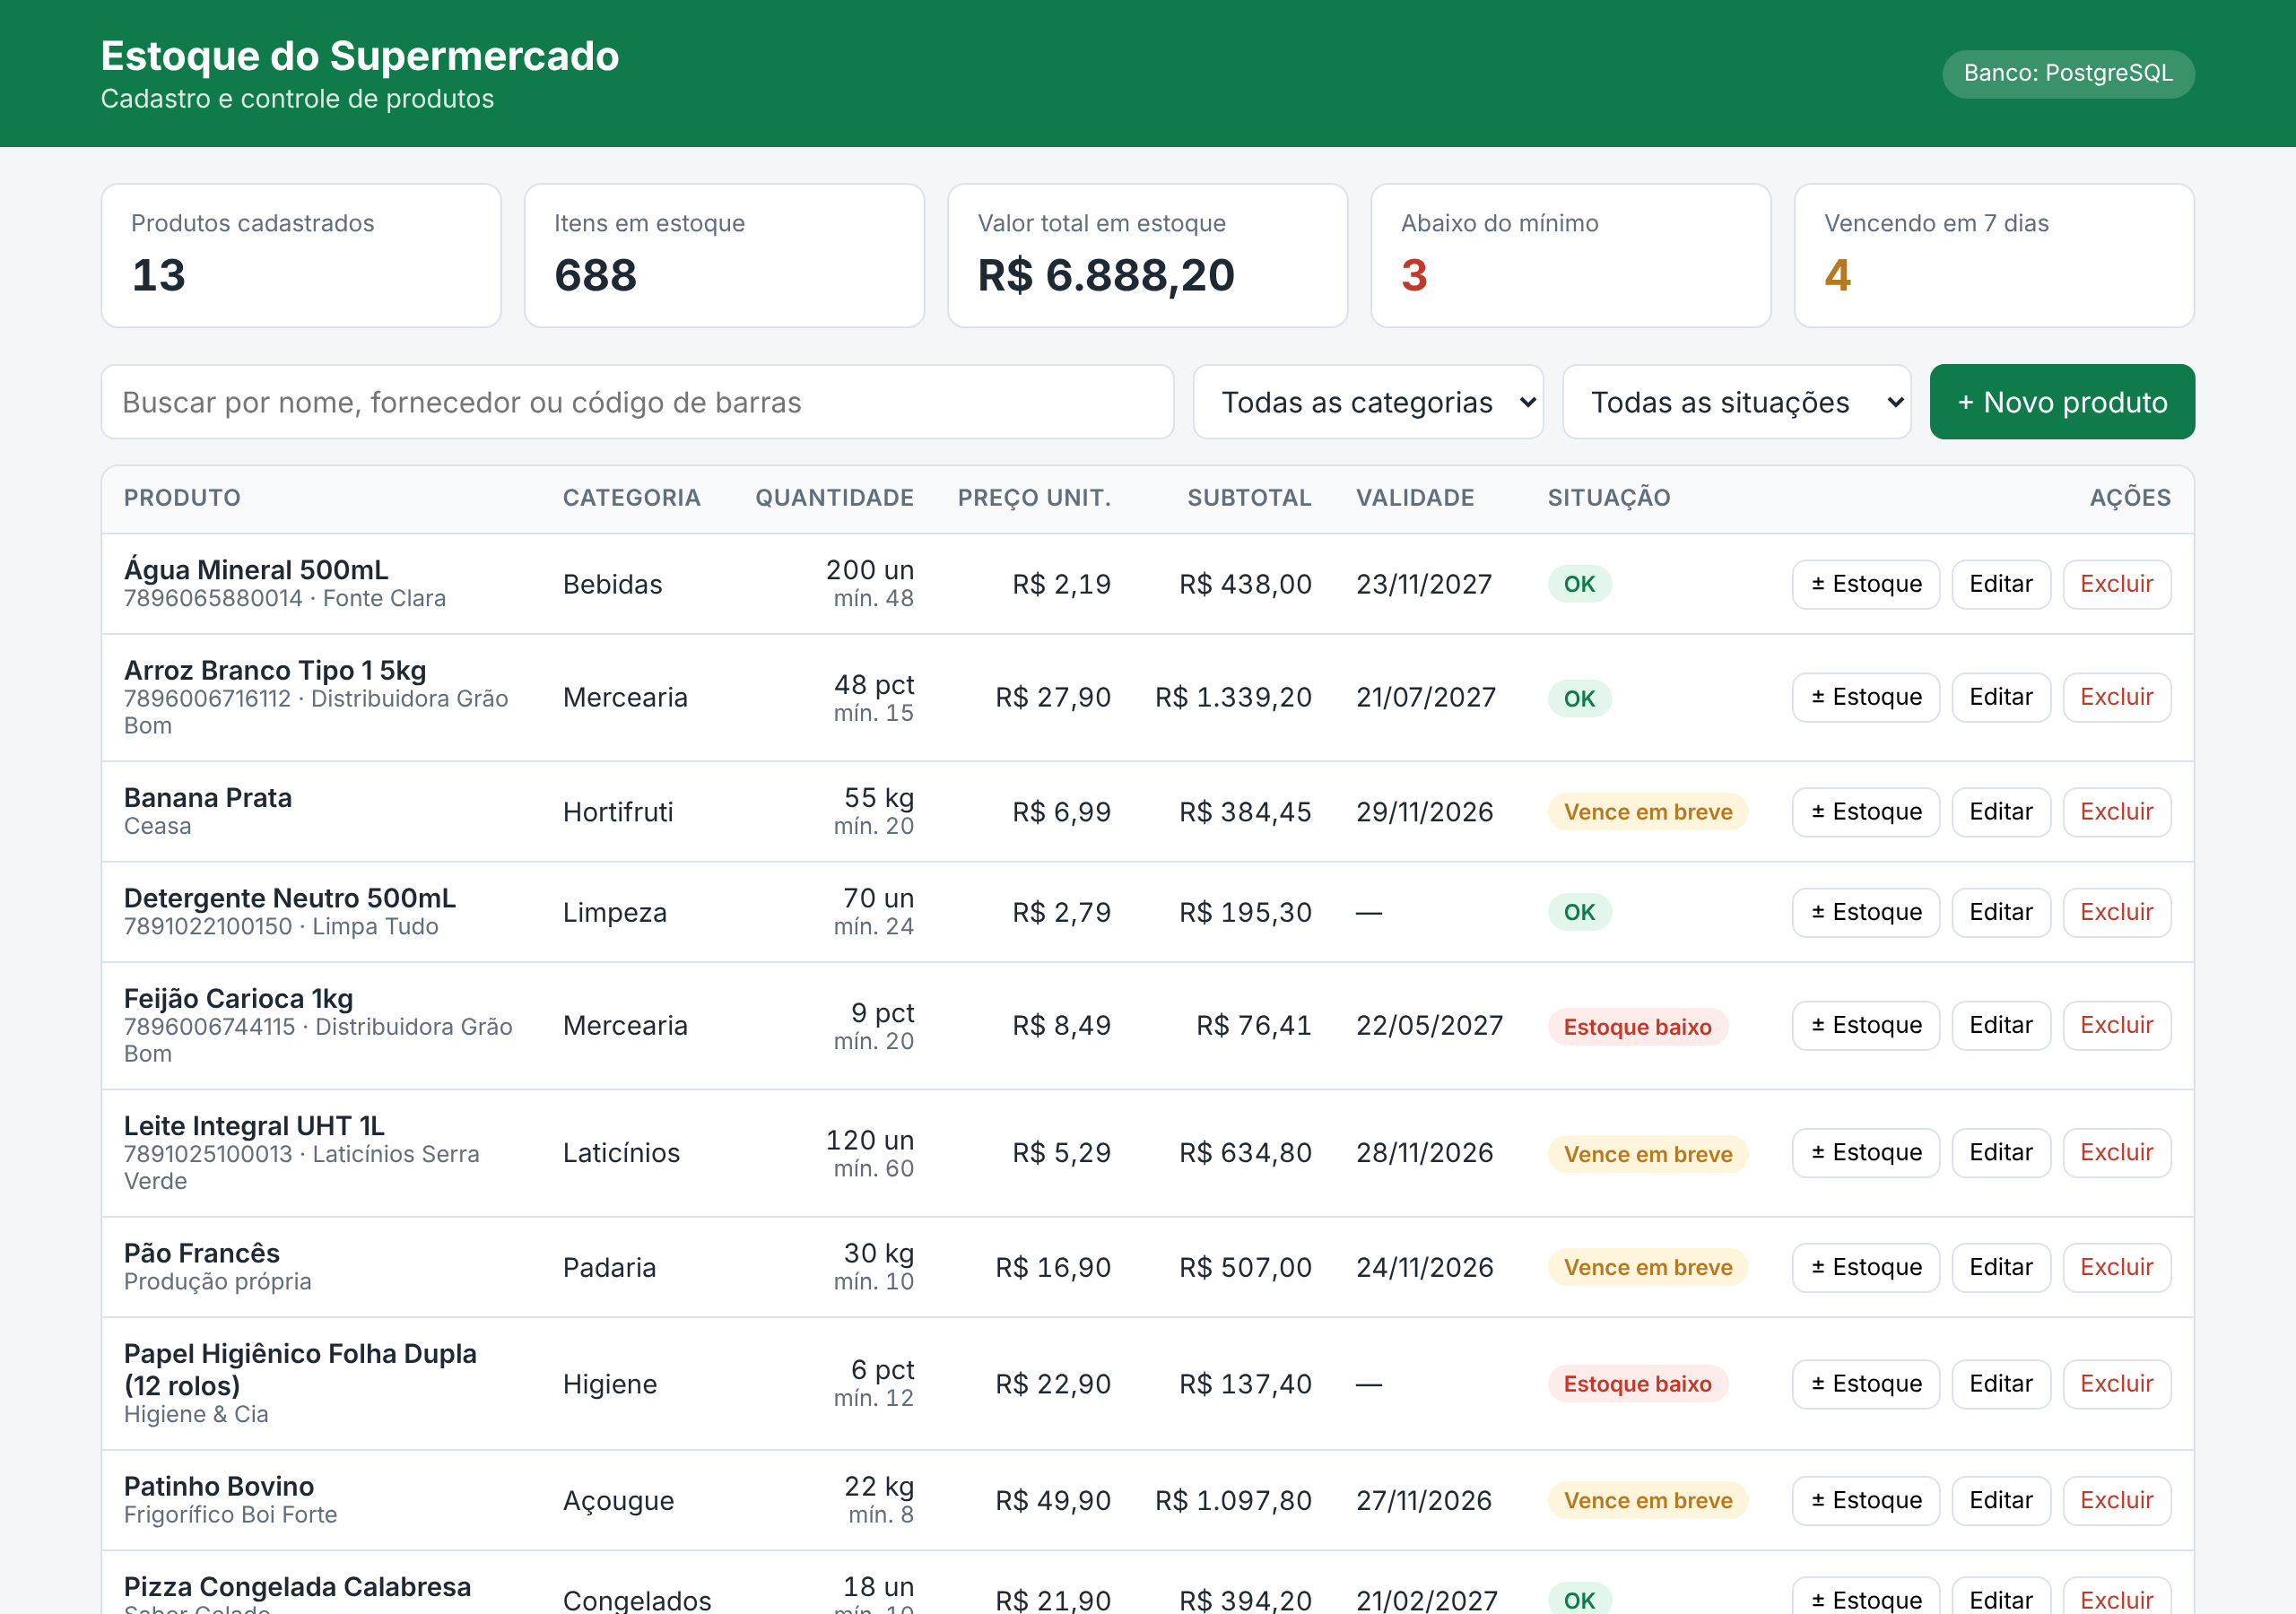
\includegraphics[width=\textwidth]{tela-principal.png}
\caption{Tela principal: indicadores, busca, filtros e lista de produtos.}
\label{fig:principal}
\end{figure}

\begin{figure}[H]
\centering
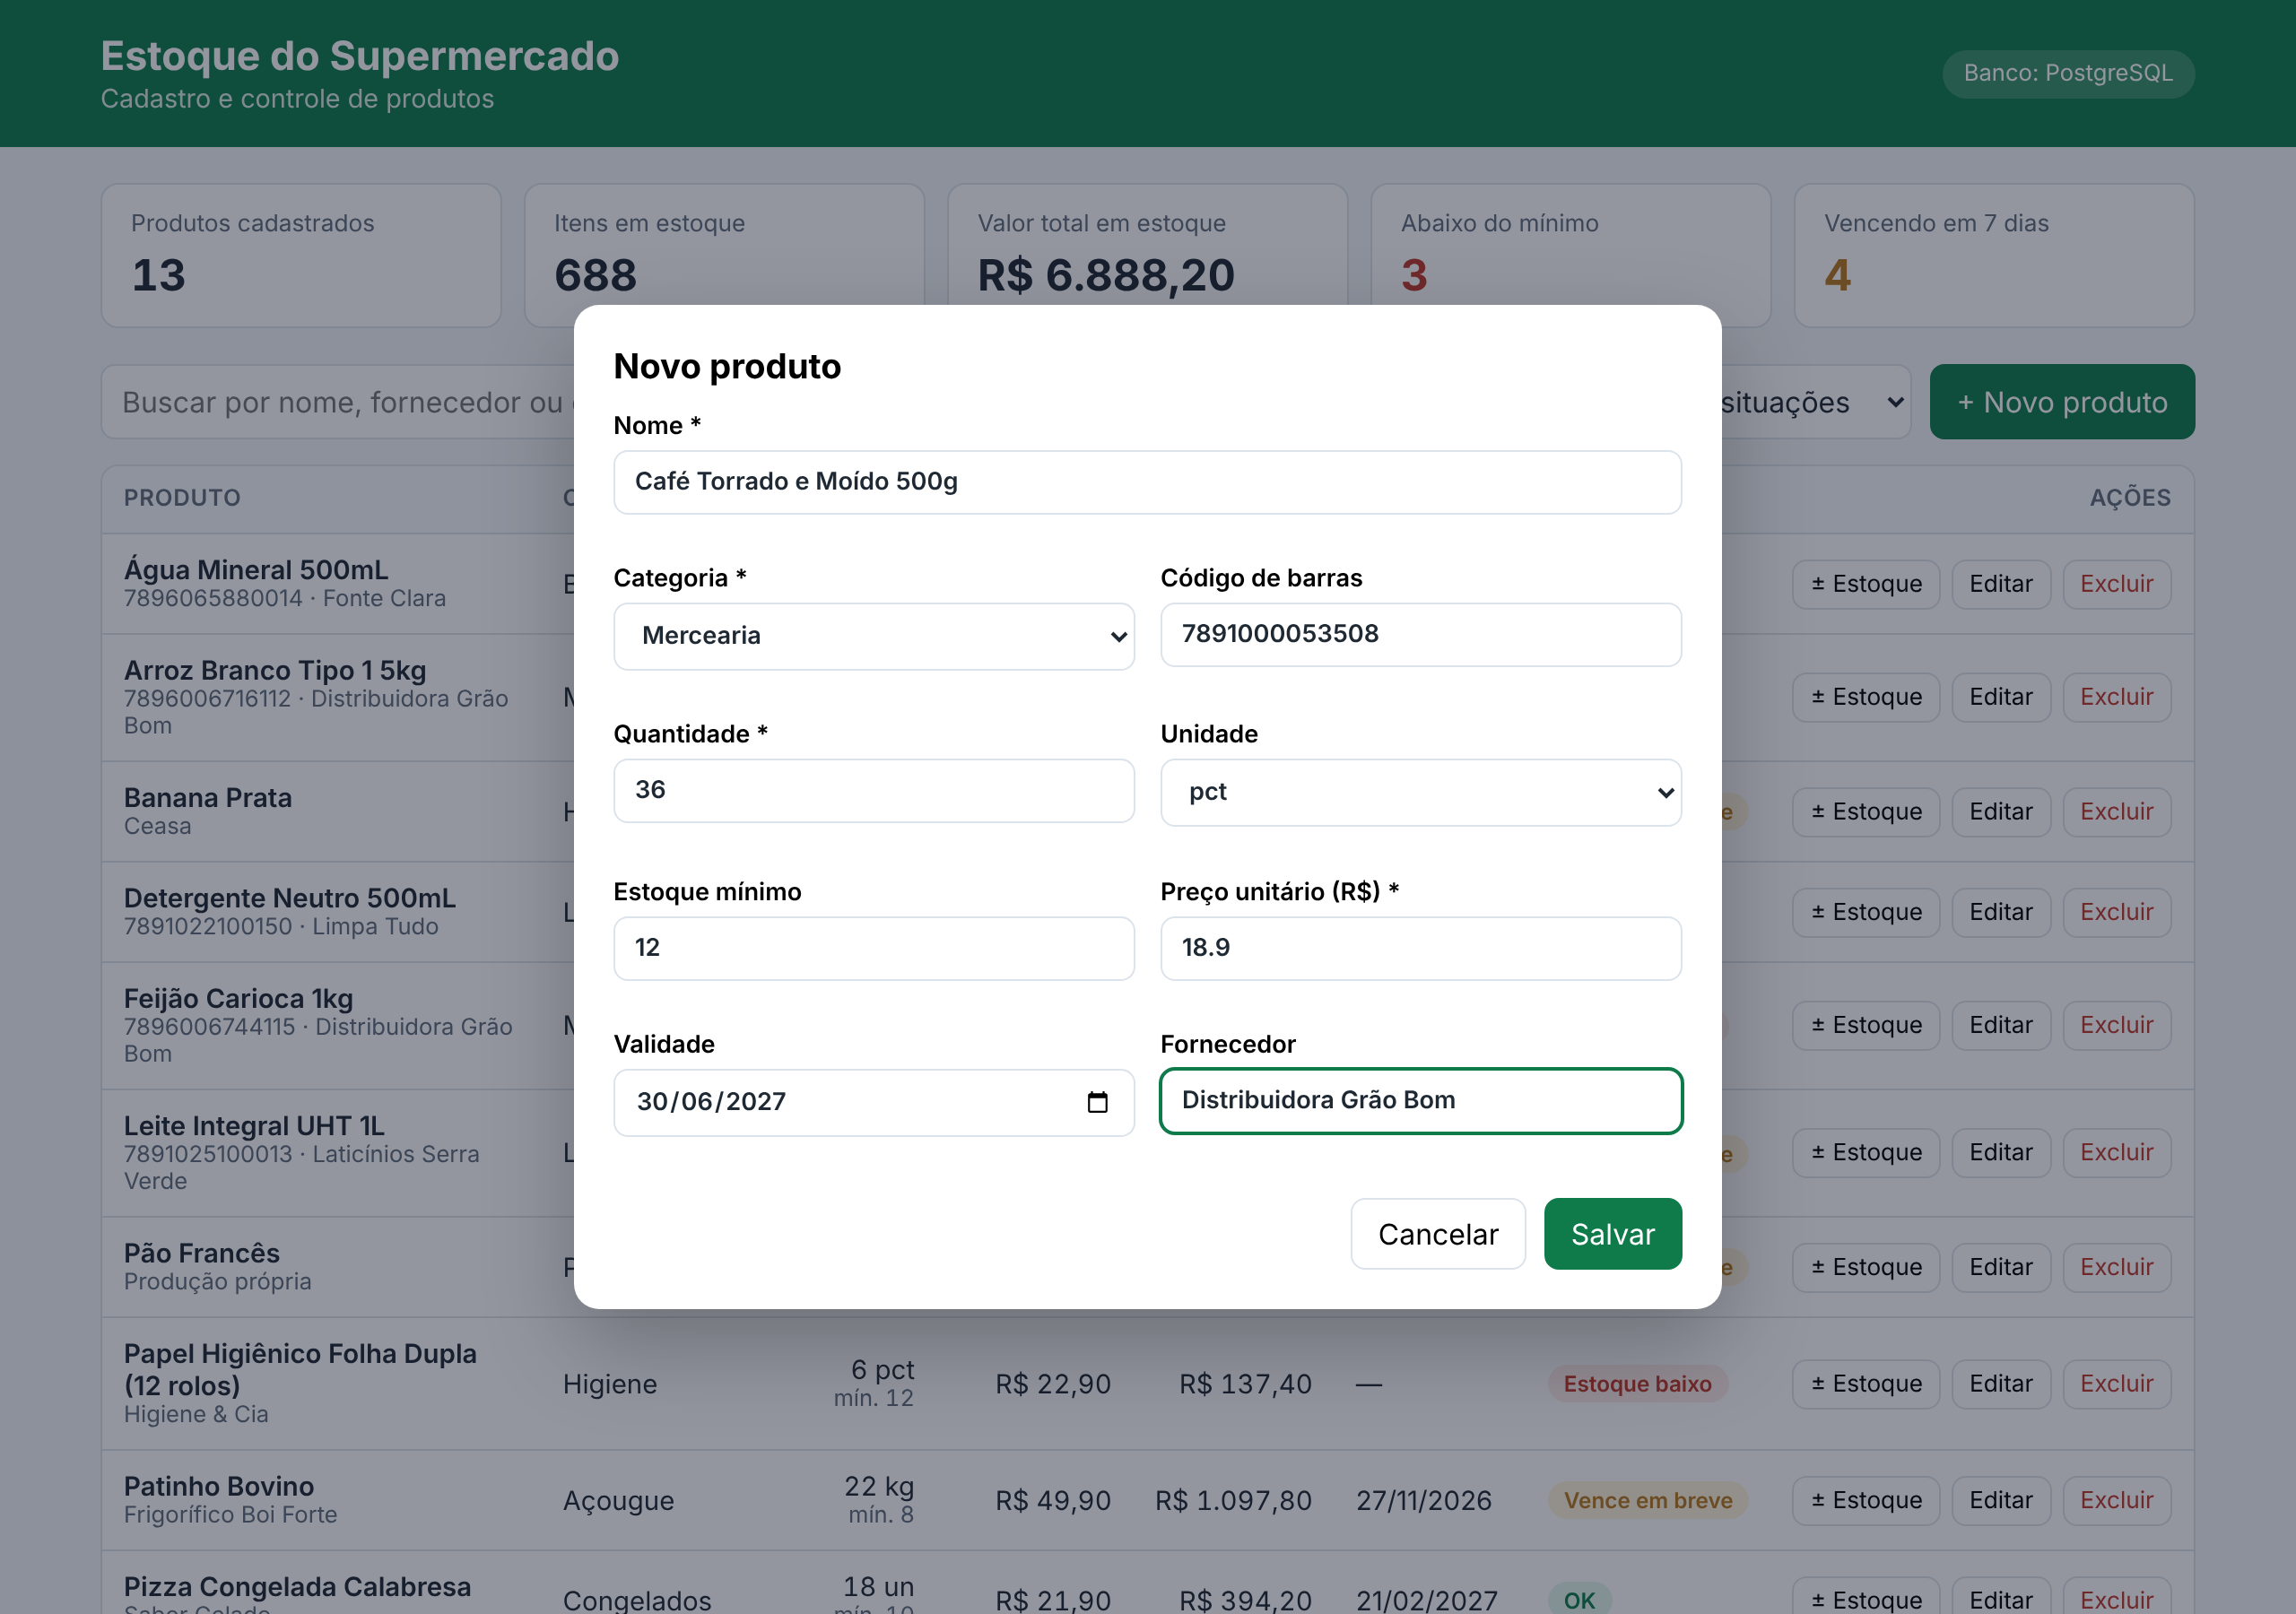
\includegraphics[width=\textwidth]{tela-cadastro.png}
\caption{Cadastro de um novo produto.}
\label{fig:cadastro}
\end{figure}

\begin{figure}[H]
\centering
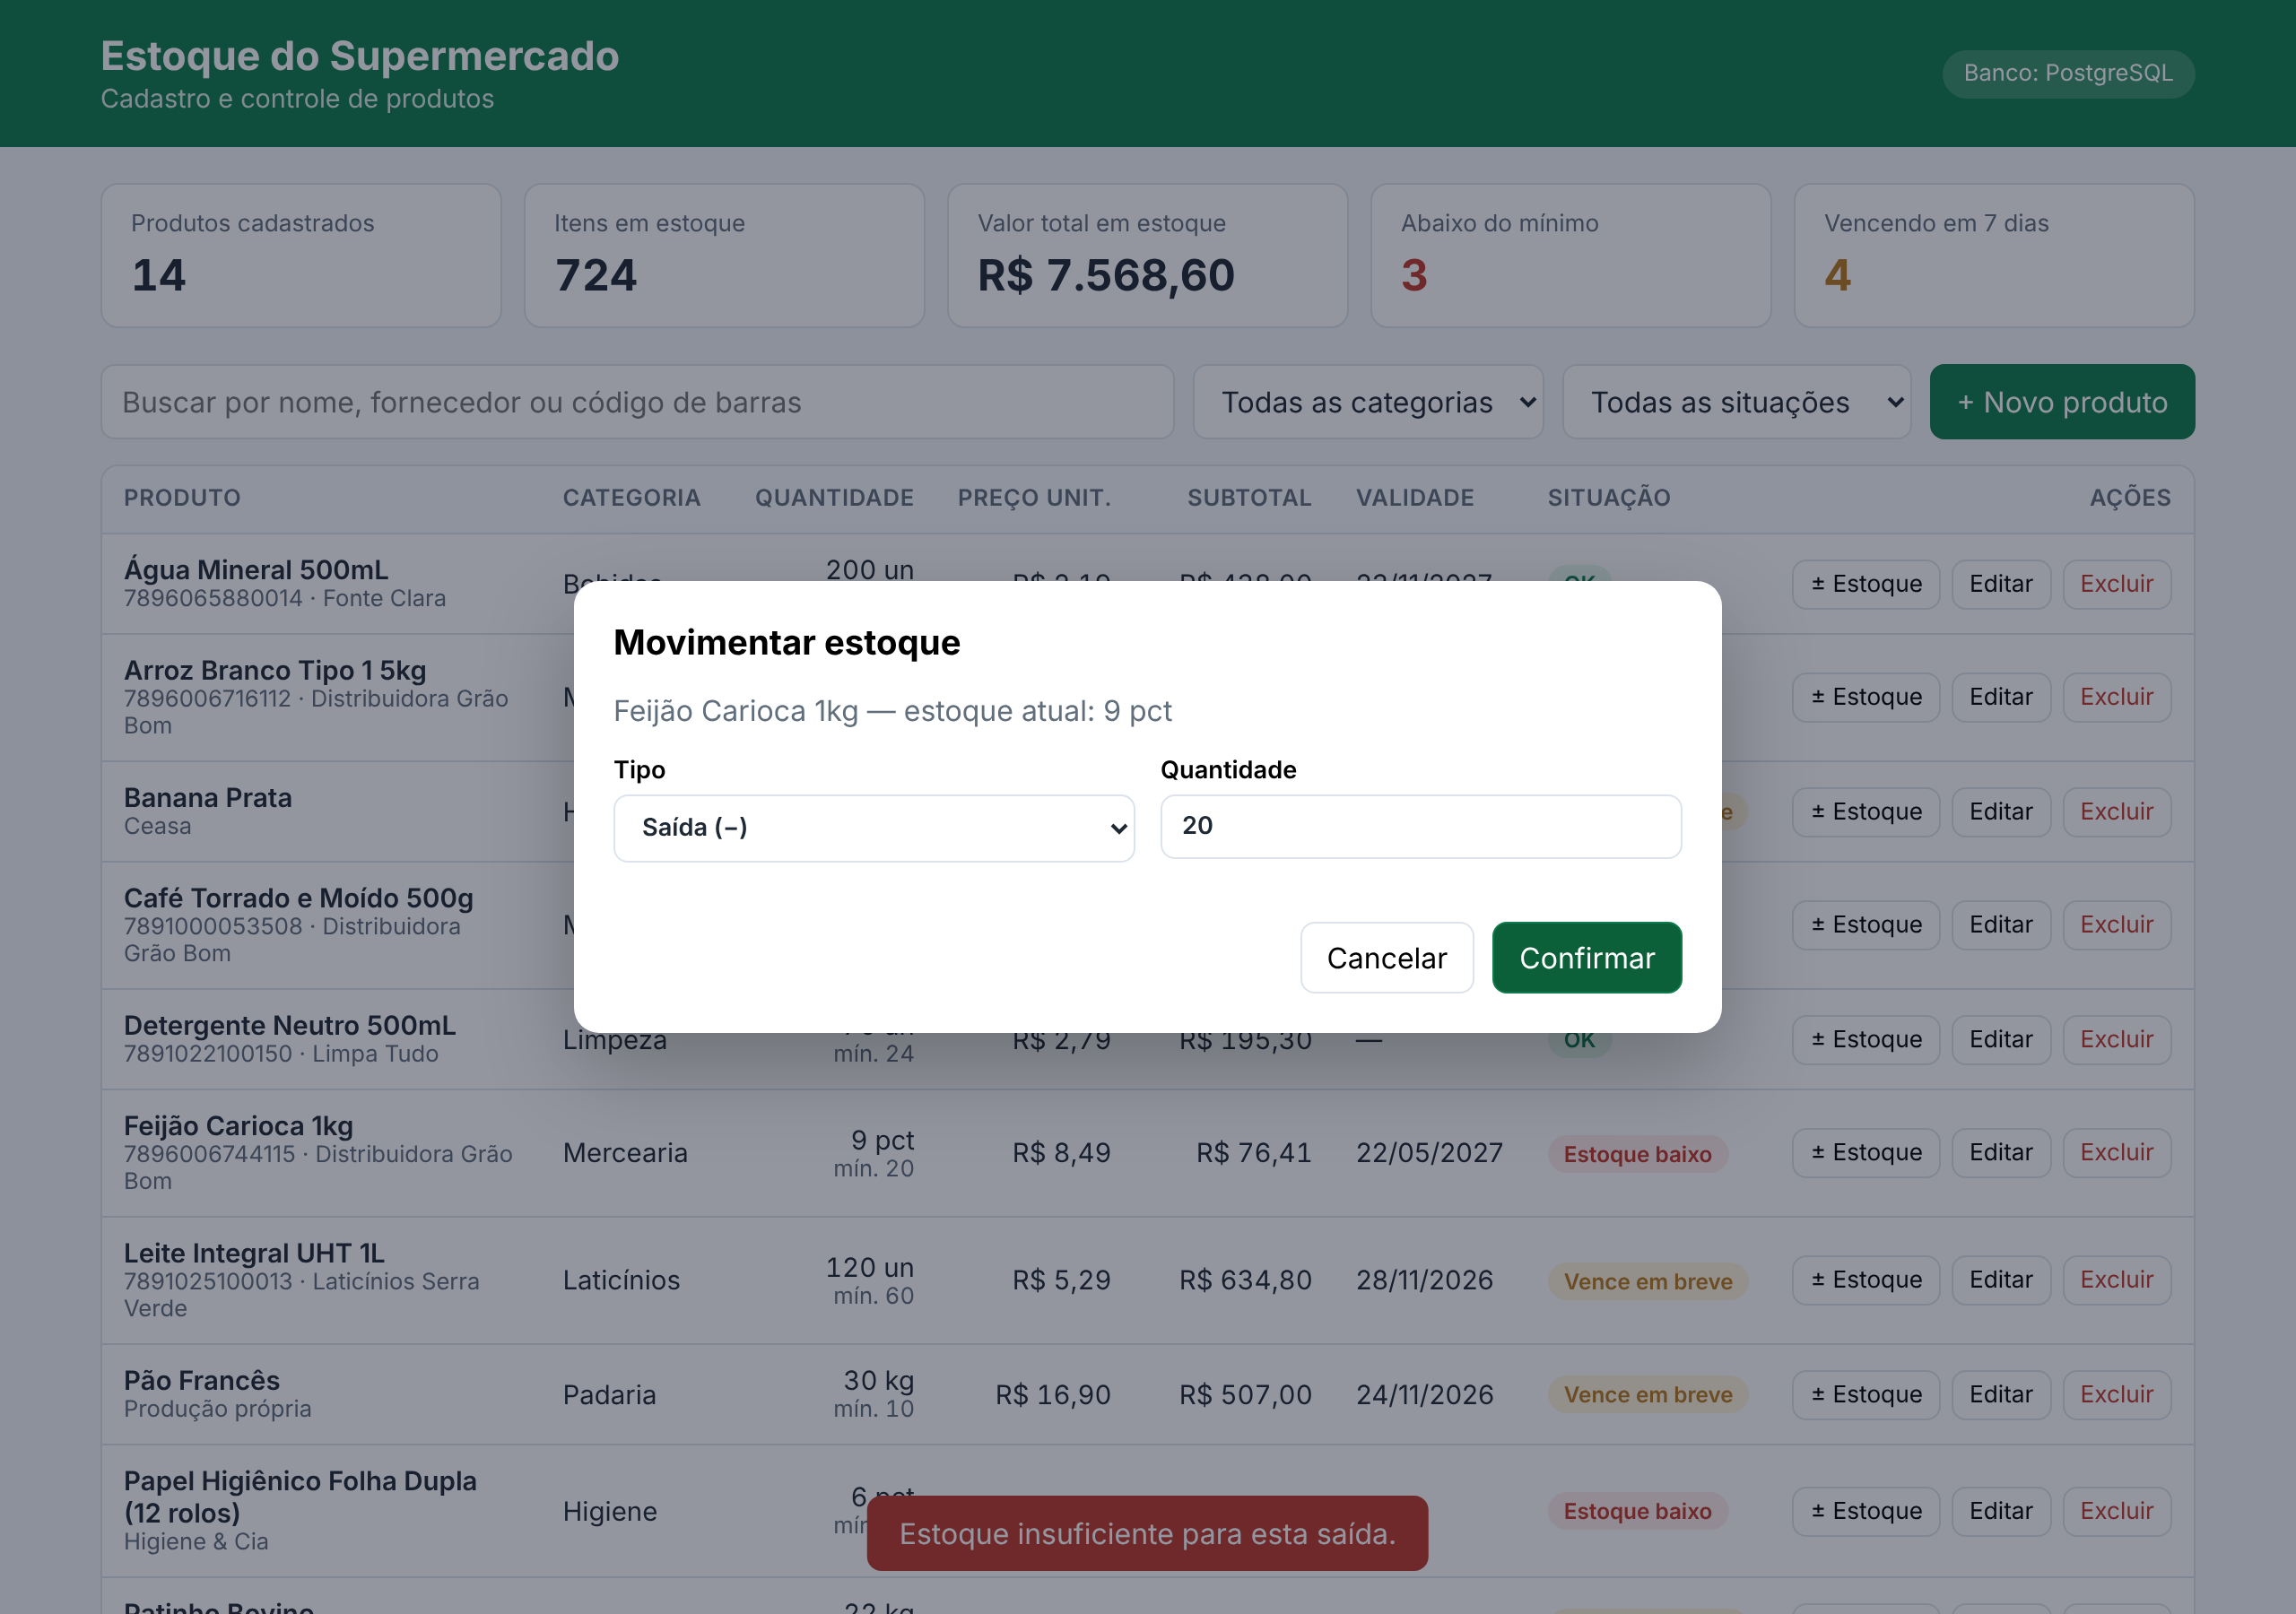
\includegraphics[width=\textwidth]{tela-estoque-insuficiente.png}
\caption{Saída de 20 unidades recusada: o produto tinha 9 em estoque.}
\label{fig:insuficiente}
\end{figure}

% =====================================================================
\section{Conclusão}
% =====================================================================

O trabalho reaproveitou o sistema de estoque desenvolvido em Computação em Nuvem, retirou o que
era específico da AWS e o preparou para o Google Cloud Run com banco no Cloud SQL. O resultado
é um sistema funcional, com finalidade clara, em que o papel do sistema operacional aparece em
situações reais de uso.

O conceito principal, a exclusão mútua contra a condição de corrida, ficou evidente no
experimento: lendo e gravando em etapas separadas, o sistema confirmou 100 vendas de um produto
com 30 unidades; com a operação atômica, o resultado foi exato. O tratamento de sinais mostrou
que, dentro de um contêiner, a forma de encerrar um processo depende de como o sistema
operacional trata o PID 1, e que um tratador simples permite ao Cloud Run desligar a aplicação
em uma fração de segundo, sem cortar requisições. A comunicação por socket Unix, a E/S
assíncrona e o isolamento em contêiner completam o quadro de como o SO está presente na
execução e na administração de uma aplicação web.

% =====================================================================
\begin{thebibliography}{9}
% =====================================================================
\bibitem{tanenbaum}
TANENBAUM, A. S.; BOS, H. \textbf{Sistemas operacionais modernos}. 4. ed. São Paulo: Pearson,
2016.

\bibitem{silberschatz}
SILBERSCHATZ, A.; GALVIN, P. B.; GAGNE, G. \textbf{Fundamentos de sistemas operacionais}.
9. ed. Rio de Janeiro: LTC, 2015.

\bibitem{postgres}
THE POSTGRESQL GLOBAL DEVELOPMENT GROUP. \textbf{PostgreSQL 16 documentation: Concurrency
Control (Transaction Isolation; Explicit Locking)}. Disponível em:
\url{https://www.postgresql.org/docs/16/mvcc.html}.

\bibitem{cloudrun}
GOOGLE CLOUD. \textbf{Cloud Run documentation: container runtime contract}. Disponível em:
\url{https://cloud.google.com/run/docs/container-contract}.

\bibitem{cloudsql}
GOOGLE CLOUD. \textbf{Connect from Cloud Run to Cloud SQL for PostgreSQL}. Disponível em:
\url{https://cloud.google.com/sql/docs/postgres/connect-run}.

\bibitem{node}
OPENJS FOUNDATION. \textbf{Node.js documentation: Process -- Signal events}. Disponível em:
\url{https://nodejs.org/api/process.html\#signal-events}.

\bibitem{pidns}
KERRISK, M. \textbf{pid\_namespaces(7)}. Linux manual page. Disponível em:
\url{https://man7.org/linux/man-pages/man7/pid_namespaces.7.html}.
\end{thebibliography}

\end{document}
